\documentclass[preprint, 10pt]{elsarticle}

\newcommand{\mcaption}[2]{\caption{\small \em #1}\label{#2}} \newcommand{\secref}[1]{\ref{#1}}
\newcommand{\Cdb}{\mbox{$\mathbb{C}$}}
\newcommand{\Rdb}{\mbox{$\mathbb{R}$}}

\newcommand{\D}{\mbox{${\mathcal D}$}}

\newcommand\numberthis{\addtocounter{equation}{1}\tag{\theequation}}
\usepackage{float}
%\usepackage{algorithmic}
%\usepackage{algorithm}
\usepackage{amsfonts}
\usepackage[fleqn,reqno]{amsmath}
\usepackage{amssymb}
%\usepackage{amsthm}
\usepackage[titletoc]{appendix}
\usepackage{array}
%\usepackage{bm}
%\usepackage{caption}
%\usepackage[usenames]{color}
\usepackage{enumitem}
%\usepackage{epsfig}
%\usepackage{fancybox}
\usepackage{filecontents}
\usepackage[top=1.2in,bottom=1.2in,left=1in, right=1in]{geometry}
\usepackage{graphics}
%%\usepackage{ifthen}
\usepackage{lineno}
%\usepackage{mathrsfs}
%\usepackage{mdframed}
%\usepackage{multirow}
%\usepackage{palatino}
%\usepackage{showkeys} %To see the labels for now.  Will remove later
%\usepackage{stmaryrd}
%\usepackage{subfigure}
%\usepackage{paralist}
\usepackage{pgfplots}
%\usepackage{tabularx}
\usepackage{tikz}
\usepackage{todonotes}
\usetikzlibrary{arrows}
\usepackage{comment}

%%%%%%  pdftex  %%%%%%%%%%%%%%%%%%%%%%%%%%%%%%%%%%%%%%%%%%%%%%%%%%%%%%
\usepackage[pagebackref=false,bookmarks=false]{hyperref} 

\hypersetup{
  bookmarksnumbered=true,
  bookmarksopen=false,
  hypertexnames=false,      
  breaklinks=true,          
  unicode=false,
  pdffitwindow=true,        
  pdfnewwindow=true,        
  colorlinks=true,         
  linkcolor=dblue,
  anchorcolor=red,
  citecolor=dorange,
  filecolor=magenta,
  urlcolor=dblue,
  pdfstartview = FitH,
  pdfkeywords = {},
  pdfcreator = {LaTeX with hyperref package}
}



\newcommand{\bd}{{\partial}}
\newcommand{\bigO}{{\mathcal{O}}}
\newcommand{\cc}{{\mathbf{c}}}
\newcommand{\DD}{{\mathcal{D}}}
\newcommand{\eeta}{{\boldsymbol\eta}}
\newcommand{\ff}{{\mathbf{f}}}
\newcommand{\grad}{{\nabla}}
\newcommand{\II}{{\mathbf{I}}}
\newcommand{\iin}{\mathrm{in}}
\newcommand{\llambda}{{\boldsymbol\lambda}}
\newcommand{\nn}{{\mathbf{n}}}
\newcommand{\NN}{{\mathcal{N}}}
\newcommand{\out}{\mathrm{out}}
\newcommand{\rr}{{\mathbf{r}}}
\newcommand{\RR}{{\mathbb{R}}}
\renewcommand{\ss}{{\mathbf{s}}}
\newcommand{\ssigma}{{\boldsymbol\sigma}}
\newcommand{\tar}{\mathrm{tar}}
\newcommand{\uu}{{\mathbf{u}}}
\newcommand{\UU}{{\mathbf{U}}}
\newcommand{\vv}{{\mathbf{v}}}
\newcommand{\xx}{{\mathbf{x}}}
\newcommand{\xxi}{{\boldsymbol{\xi}}}
\newcommand{\yy}{{\mathbf{y}}}

\def\gap{\hspace*{.2in}}

% Derivatives
\newcommand{\pderiv}[2]{\frac{\partial #1}{\partial #2}}
\newcommand{\tderiv}[2]{\frac{d #1}{d #2}}
\newcommand{\ppd}[2]{\frac{\partial^2 #1}{{\partial #2}^2}}

% Nick's commands
\newcommand{\vsp}[1]{\vspace{#1 pc} \noindent}
\newcommand{\abs}[1]{\lvert #1 \rvert}
\newcommand{\mean}[1]{\left< #1 \right>}
\newcommand{\thL}{$\theta$--$L$}
\newcommand{\eps}{\varepsilon}
\newcommand{\Vn}{V_n}
\newcommand{\Vs}{V_s}
\newcommand{\atau}{\abs{\tau}}
\newcommand{\thalpha}{\pderiv{\theta}{\alpha}}
\newcommand{\elfun}{\zeta}
\newcommand{\thhat}{\hat{\theta}}
\newcommand{\Dt}{\Delta t}
\newcommand{\NLterm}{\mathcal{N}}
\newcommand{\Mterm}{\mathcal{M}}
\newcommand{\FourierSum}{ \sum_{k = -N_\iin /2}^{N_\iin /2-1} }
\newcommand{\atausig}{\atau^{(\sigma)}}
\newcommand{\Vnsig}{\Vn^{(\sigma)}}
\newcommand{\Vssig}{\Vs^{(\sigma)}}


\newcommand{\tauD}[1]{\tau_{#1\text{D}}}
\newcommand{\atauD}[1]{\abs{\tau_{#1\text{D}}}}

\begin{document}

\title{Viscous Transport in Eroding Porous Media}


% OTHER TITLE POSSIBILITIES
% Viscous Erosion in Porous Media (change 'in' to 'of'?)
% A fast and accurate method for viscous erosion of a 2D porous medium
% A boundary-integral method for viscous erosion of a porous medium
% A computational framework to simulate the viscous erosion of a porous medium

\author[SH]{Shang-Huan Chiu}
\author[Nick]{M.~Nicholas J.~Moore}
\author[Bryan]{Bryan D.~Quaife}

\address[SH]{Department of Scientific Computing, Florida State
University, Tallahassee, FL, 32306.}
\address[Nick]{Department of Mathematics and Geophysical Fluid Dynamics Institute, Florida State University, Tallahassee, FL, 32306.}
\address[Bryan]{Department of Scientific Computing and Geophysical Fluid Dynamics Institute, Florida State University, Tallahassee, FL, 32306.}

\begin{abstract} 
  An abstract
\end{abstract}

\begin{keyword}
  Keyword 1 \sep Keyword 2 \sep Keyword 3 
\end{keyword}

\maketitle

%%%%%%%%%%%%%%%%%%%%%%%%%%%%%%%%%%%%%%%%%%%%%%%%%%%%%%%%%%%%%%%%%%%%%%%
\section{Introduction}
\label{s:intro}
%%%%%%%%%%%%%%%%%%%%%%%%%%%%%%%%%%%%%%%%%%%%%%%%%%%%%%%%%%%%%%%%%%%%%%%
A continuation of the methods paper~\cite{qua-moo2018}.
\paragraph{Governing Equations}
\begin{equation}
\label{eqn:erosionModel}
\begin{split}
  \mu \Delta \uu = \grad p, &\hspace{20pt} \xx \in \Omega, \gap &&\mbox{\em conservation
of momentum}\\
\grad \cdot \uu = 0, &\hspace{20pt} \xx \in \Omega, \gap &&\mbox{\em conservation of mass} \\
\uu = 0, &\hspace{20pt} \xx \in \gamma, \gap &&\mbox{\em no slip on the
bodies} \\
\uu = \UU, &\hspace{20pt} \xx \in \Gamma, \gap &&\mbox{\em outer wall
velocity} \\
\Vn = \CE \, \abs{\tau}, &\hspace{20pt} \xx \in \gamma,
&&\mbox{\em erosion model}.
\end{split}
\end{equation}



%%%%%%%%%%%%%%%%%%%%%%%%%%%%%%%%%%%%%%%%%%%%%%%%%%%%%%%%%%%%%%%%%%%%%%%
\paragraph{Contributions}
\begin{itemize}
  \item Use novel near-singular Barycentric integration scheme for
    Stokes equation outlined in~\cite{bar-wu-vee2015}.
  \item Need to compute one additional derivative since we need the
    derivative of the velocity to find the vorticity and stress tensor
  \item Tracer trajectories at different time steps
  \item Compute the anomalous diffusion rate using similar techniques as
    the paper with Pietro~\cite{dea-qua-bir-jua2018}
  \item Need a novel way to do time stepping through the complex
    geometry
\end{itemize}

\paragraph{Limitations}
\begin{itemize}
  \item Bodies are still pinned
  \item Bodies are still two dimensional
\end{itemize}

\paragraph{Related Work}

%%%%%%%%%%%%%%%%%%%%%%%%%%%%%%%%%%%%%%%%%%%%%%%%%%%%%%%%%%%%%%%%%%%%%%%
\paragraph{Outline of the Paper}

%%%%%%%%%%%%%%%%%%%%%%%%%%%%%%%%%%%%%%%%%%%%%%%%%%%%%%%%%%%%%%%%%%%%%%%
\section{Boundary Integral Equation Formulation}
\label{s:formulation}
Continuing on our previous work~\cite{qua-moo2018}, we use a completed
double-layer potential formulation for the velocity $\uu$.  The
double-layer potential is
\begin{align}
  \DDD[\eeta](\xx) = \frac{1}{\pi}\int_{\bd\Omega} 
    \frac{\rr \cdot \nn}{\rho^2} \frac{\rr \otimes \rr}{\rho^2}
    \eeta(\yy) ds_\yy,
\end{align}
where $\rr = \xx - \yy$, $\rho = \|\rr\|$, and $\eeta$ is an unknown
density function.  The double-layer potential itself can not represent
all solutions of the incompressible Stokes equations.  Therefore, we
complete the integral equation formulation following the work of Power
and Miranda~\cite{pow-mir1987}.  The completion depends on the
Stokeslets and rotlets
\begin{align}
  S[\llambda_\ell,\cc_\ell](\xx) = \frac{1}{4\pi} \left( 
    -\log \rho \II + \frac{\rr \otimes \rr}{\rho^2} \right), \qquad
  R[\xi_\ell,\cc_\ell](\xx) = \frac{\rr^\perp}{\rho^2} \xi_\ell,
\end{align}
where $\rr = \xx - \cc_\ell$, $\cc_\ell$ is a point inside the
$\ell^{th}$ eroding body, $\rr^\perp = (r_2,-r_1)$, and $\rho =
\|\rr\|$.  Then, the solution of the Stokes equation is
\begin{align}
  \uu(\xx) = \DDD[\eeta](\xx) + 
    \sum_{\ell=1}^M S[\llambda_\ell,\cc_\ell](\xx) + 
    \sum_{\ell=1}^M R[\xi_\ell,\cc_\ell](\xx),
\end{align}
where the density function, Stokeslets, and rotlets satisfy
\begin{align}
  \ff(\xx) &= -\frac{1}{2}\eeta(\xx) + \DDD[\eeta](\xx) + 
    \sum_{\ell=1}^M S[\llambda_\ell,\cc_\ell](\xx) + 
    \sum_{\ell=1}^M R[\xi_\ell,\cc_\ell](\xx) +
    \NN_0(\eeta](\xx), \qquad \xx \in \bd\Omega, \\
  \lambda_\ell &= \frac{1}{2\pi} \int_{\gamma_\ell} 
    \eeta(\yy) ds_\yy \qquad \ell = 1,\ldots,M, \\
  \xi_\ell &= \frac{1}{2\pi} \int_{\gamma_\ell}
    (\yy - \cc_\ell)^\perp  \eeta(\yy) ds_\yy 
    \qquad \ell = 1,\ldots,M.
\end{align}

We will apply a quadrature rule that requires that the double-layer
potential representations of the velocity, shear stress, pressure, and
vorticity are written in terms of the Cauchy integral and its first two
derivatives
\begin{align}
  \label{eqn:Cauchy}
  v(x) &= \frac{1}{2\pi i} \int_\Gamma 
    \frac{\tau(y)}{x - y} dy, \\
  v'(x) &= -\frac{1}{2\pi i} \int_\Gamma 
    \frac{\tau(y)}{(x - y)^2} dy, \\
  v''(x) &= \frac{2}{2\pi i} \int_\Gamma 
    \frac{\tau(y)}{(x - y)^3} dy.
\end{align}

%%%%%%%%%%%%%%%%%%%%%%%%%%%%%%%%%%%%%%%%%%%%%%%%%%%%%%%%%%%%%%%%%%%%%%%
\subsection{Cauchy Integral Representation of the Velocity}
The Stokes double-layer potential can be written as
\begin{align}
  \DDD[\eeta](\xx) &= 
    \frac{1}{2\pi} \int_{\Gamma} 
      \frac{\nn}{\rho^2} (\rr \cdot \eeta) ds_\yy + 
    \frac{1}{2\pi} \nabla \int_{\Gamma}
      \frac{\rr \cdot \nn}{\rho^2} (\yy \cdot \eeta)ds_\yy \\
    &- \frac{1}{2\pi} x_1 \nabla \int_{\Gamma}
      \frac{\rr \cdot \nn}{\rho^2}\eta_1(\yy) ds_\yy -
    \frac{1}{2\pi} x_2 \nabla \int_{\Gamma}
      \frac{\rr \cdot \nn}{\rho^2}\eta_2(\yy) ds_\yy,
\end{align}
and this formulation is convenient since each of the integrals can be
written as a Laplacian double-layer potential,
\begin{align}
  \DD[\tau](\xx) = -\frac{1}{2\pi} \int_{\Gamma} \pderiv{}{\nn_\yy}
    \log(\rho) \tau(\yy) ds_\yy.
\end{align}
Finally, by identifying $\RR^2$ with $\CC$, for purely real $\tau$, the
Laplacian double-layer potential can be written as the real part of a
Cauchy integral
\begin{align}
  \DD[\tau](x) = \Re (v(x)),
  \qquad \text{where} \qquad
  v(x) = \frac{1}{2\pi i} \int_\Gamma \frac{\tau(y)}{x - y} dy.
\end{align}
Therefore, the Stokes double-layer potential can be written as five
Cauchy integrals and their derivatives with the density functions $\yy
\cdot {\color{red}\eeta}$, $\eta_1$, and $\eta_2,$
{\color{red}
\begin{align}
 u_1(\xx)&= \Re (v[\tau_1](x)) + \Re (v'[\yy\cdot\eeta](x)) 
           -x_1\Re (v'[\eta_1](x)) -x_2\Re (v'[\eta_2](x)),\\
 u_2(\xx)&= \Re (v[\tau_2](x)) - \operatorname{Im} (v'[\yy\cdot\eeta](x)) 
       +x_1\operatorname{Im} (v'[\eta_1](x)) 
      +x_2\operatorname{Im} (v'[\eta_2](x)),
\end{align}
where
\begin{align*} 
\DD[\eeta](\xx)=(u_1(\xx),u_2(\xx)), \,\, 
\xx=(x_1,x_2), \,\,
\tau_1=(\eta_1+i\eta_2)\frac{\Re \, n}{n}, \text{ and }
\tau_2=(\eta_1+i\eta_2)\frac{\operatorname{Im} n}{n}.
\end{align*}
}
%%%%%%%%%%%%%%%%%%%%%%%%%%%%%%%%%%%%%%%%%%%%%%%%%%%%%%%%%%%%%%%%%%%%%%%
\subsection{Cauchy Integral Representation of the Shear Stress}
Since the rate of erosion is proportional to the shear stress, we also
require the gradient of the Stokes double-layer potential $\nabla
\DDD[\eeta](\xx)$.  Using the Cauchy integral formulation, the gradient
of of the double-layer potential velocity is
{\color{red}
\begin{align}
 \nabla\D[\eeta] (\xx)=
\left[
\begin{matrix}
\displaystyle\frac{\partial u_1(\xx)}{\partial x_1} & 
\displaystyle\frac{\partial u_1(\xx)}{\partial x_2}\\ \\
\displaystyle\frac{\partial u_2(\xx)}{\partial x_1} & 
\displaystyle\frac{\partial u_2(\xx)}{\partial x_2}
\end{matrix}
\right],
\end{align}
where 
\begin{align}
\frac{\partial u_1(\xx)}{\partial x_1}&= \Re (v'[\tau_1](x)) + \Re (v''[\yy\cdot\eeta](x)) 
           -\Re (v'[\eta_1](x)) -x_1\Re (v''[\eta_1](x))-x_2\Re (v''[\eta_2](x)),\\
\frac{\partial u_1(\xx)}{\partial x_2}&= - \operatorname{Im} (v'[\tau_1](x)) 
      - \operatorname{Im} (v''[\yy\cdot\eeta](x)) 
       +x_1\operatorname{Im} (v''[\eta_1](x)) 
       -\Re (v'[\eta_2](x))
      +x_2\operatorname{Im} (v''[\eta_2](x)),\\
\frac{\partial u_2(\xx)}{\partial x_1}&= \Re (v'[\tau_2](x)) 
      -\operatorname{Im} (v''[\yy\cdot\eeta](x)) 
       +\operatorname{Im} (v'[\eta_1](x))
       +x_1\operatorname{Im} (v''[\eta_1](x)) 
      +x_2\operatorname{Im} (v''[\eta_2](x)),\\
\frac{\partial u_2(\xx)}{\partial x_2}&= -\operatorname{Im} (v'[\tau_2](x)) 
      -\Re (v''[\yy\cdot\eeta](x)) 
       +x_1\Re (v''[\eta_1](x)) 
      +\operatorname{Im} (v'[\eta_2](x)
      +x_2\Re (v''[\eta_2](x)).
\end{align}
}
%\begin{align}
%  \nabla\D[\eeta](\xx) = \frac{1}{2\pi}\nabla\int_{\Gamma}
%    &\frac{\nn}{\rho^2}(\rr \cdot \eeta)ds_\yy +
%  \frac{1}{2\pi}\nabla\nabla\int_{\Gamma}
%    \frac{\rr \cdot \nn}{\rho^2}({\yy} \cdot\eeta) ds_y \\
%  &- \frac{1}{2\pi} \nabla x_1 \nabla \int_{\Gamma}
%      \frac{\rr \cdot \nn}{\rho^2}\eta_1(\yy) ds_\yy -
%  \frac{1}{2\pi} \nabla x_2 \nabla \int_{\Gamma}
%      \frac{\rr \cdot \nn}{\rho^2}\eta_2(\yy) ds_\yy.
%\end{align}
Then, the deformation tensor can be written in terms of Cauchy integrals
\todo[inline]{For S-H to fill in}
\begin{align}
  \ssigma = \frac{1}{2} 
    \left(\nabla \DDD[\eeta] + \nabla^T \DDD[\eeta] \right) 
      \nn \cdot \ss = \ldots
\end{align}

%%%%%%%%%%%%%%%%%%%%%%%%%%%%%%%%%%%%%%%%%%%%%%%%%%%%%%%%%%%%%%%%%%%%%%%
\subsection{Cauchy Integral Representation of the Vorticity}

%%%%%%%%%%%%%%%%%%%%%%%%%%%%%%%%%%%%%%%%%%%%%%%%%%%%%%%%%%%%%%%%%%%%%%%
\subsection{Cauchy Integral Representation of the Pressure}




%%%%%%%%%%%%%%%%%%%%%%%%%%%%%%%%%%%%%%%%%%%%%%%%%%%%%%%%%%%%%%%%%%%%%%%
\section{Transport, Tracers, and Tortuosity}
%%%%%%%%%%%%%%%%%%%%%%%%%%%%%%%%%%%%%%%%%%%%%%%%%%%%%%%%%%%%%%%%%%%%%%%
Erosion leads to interesting porous geometries, and we are interested in
characterizing transport in these geometries.  To characterize the
transport, we first require tracer trajectories (streamlines) that are
governed by
\begin{align}
  \frac{d\ss}{dt} = \uu(\ss,t), \quad \ss(0) = \ss_0.
\end{align}
Instead of allowing the transport and erosion to happen simultaneously,
we freeze the geometry and compute the streamlines in this fixed
geometry.  Therefore, the velocity $\uu$ has no temporal dependence when
we characterize the transport.

The tortuosity measures ...


%%%%%%%%%%%%%%%%%%%%%%%%%%%%%%%%%%%%%%%%%%%%%%%%%%%%%%%%%%%%%%%%%%%%%%%
\section{Numerical Methods}
\label{s:method}
%%%%%%%%%%%%%%%%%%%%%%%%%%%%%%%%%%%%%%%%%%%%%%%%%%%%%%%%%%%%%%%%%%%%%%%
A standard discretization of these equations approximates the
double-layer potential with the trapezoid rule.  This quadrature rule is
appropriate if the integrands are sufficiently smooth, where the
smoothness depends on the number of discretization points.  However,
given a fixed resolution, if the target point $\xx$ is too close to $\bd
\Omega$, the trapezoid rule becomes inaccurate and the overall method
becomes unstable.  There have been a variety of near-singular
integration schemes developed, and we extend a method first outlined by
Barnett et al.~\cite{bar-wu-vee2015} which we will call the {\em
Barycentric quadrature rule}.  Here, we briefly describe this quadrature
method, and then derive a necessary extension to simulate erosion.

Since we are able to write on all our quantities of interest in terms of
a Cauchy integral and its derivatives, we only require a near-singular
integration method for equation~\eqref{eqn:Cauchy}.  A quadrature scheme
for $v(x)$, for a target point $x$, is
\begin{align}
  v(x) \approx \frac{1}{2\pi i} \sum_{j=1}^N 
    w_j \frac{\tau(y_j)}{x - y_j},
\end{align}
where $w_j$ are the quadrature weights and $y_j \in \Gamma$ are the
quadrature nodes.  If the trapezoid rule is used, the quadrature rule
has spectral accuracy.  However, for a fixed resolution $N$, the error
grows without bound as $x$ approaches $\Gamma$.  As outline by Barnett
et al.~\cite{bar-wu-vee2015}, the error is uniformly bounded if the
Barycentric quadrature rule
\begin{align}
  v(x) \approx \frac{\sum\limits_{j=1}^N \frac{v_j^-}{y_j-x}w_j}
    {\sum\limits_{j=1}^N \frac{1}{y_j-x}w_j},  \qquad
  v'(x) \approx \frac{\sum\limits_{j=1}^N \frac{v_j^- - v(x)}{(y_j - x)^2}w_j}
    {\sum\limits_{j=1}^N \frac{1}{y_j-x}w_j}, 
\end{align}
is used, where $x$ is a target point that is interior to $\Gamma$,
and $v_j^-$ is the value of $v(y_j)$.  Modifications of this formula
exist if $x$ is exterior to $\Gamma$.

%%%%%%%%%%%%%%%%%%%%%%%%%%%%%%%%%%%%%%%%%%%%%%%%%%%%%%%%%%%%%%%%%%%%%%%%
\subsection{Barycentric Quadrature for $v''(x)$}
In order to simulate erosion, we require the deformation gradient which
means that a quadrature rule for $v''(x)$ is required.  Using the same
techniques that are used to compute $v(x)$ and $v'(x)$, a Barycentric
quadrature rule for the second derivative can be constructed using the
identities
{\color{red}
\begin{alignat}{3}
  0 &= \frac{1}{2\pi i}\int_{\Gamma} 
    \frac{2v^-({ y})-2v(x)-2(y-x)v'(x)-(y-x)^2v''(x)}{(y-x)^3} dy, &&x \in \Omega, \\
  0 &= \frac{1}{2\pi i}\int_{\Gamma}
    \frac{2v^+(y)-2v(x)-2(y-x)v'(x)-(y-a)^{-1}(x-a)(y-x)^2 v''(x)}
    {(y-x)^3} dy, \quad &&x \in \Omega^c.  \label{eqn:Identity}
\end{alignat}
and the quadrature formulations are
\begin{alignat}{3}
  v''(x) &\approx
    \frac{2\sum\limits_{j=1}^N \frac{v_j^- -v(x)-(y_j-x)v'(x)}{(y_j-x)^3}w_j}
    {\sum\limits_{j=1}^N \frac{1}{y_j-x}w_j}, &&x \in \Omega, \\
  v''(x) &\approx \frac{1}{x-a}\frac{2\sum\limits_{j=1}^N
    \frac{v_j^+ -v(x)-(y_j-x)v'(x)}{(y_j-x)^3}}{\sum\limits_{j=1}^N \frac{(y_j-a)^{-1}}{y_j-x}w_j}
    , \quad &&x \in \Omega^c.  \label{eqn:SecondBary}
\end{alignat}
where $a$ is a point inside the $\Omega$ in equations~\eqref{eqn:Identity} and \eqref{eqn:SecondBary}.

}


%%%%%%%%%%%%%%%%%%%%%%%%%%%%%%%%%%%%%%%%%%%%%%%%%%%%%%%%%%%%%%%%%%%%%%%
\subsection{Fast Summation Methods}
\label{sec:fmm}

{\color{red}
By using Barycentric quadrature rule to approach integrations, we get a reasonable(?) double-layer potential and quantities of interest at target points but it requires $\mathcal{O}(N^2)$ operations per target point which is computational expensive if we impose it on all the target points. In order to accelerate the process and keep the accuracy, it is a compromise that we use Barycentric quadrature rule to approach the nearly singular integratons but apply trapezoid rule when the target point is far from source points. 


To numerically compute the completed double-layer potential, we discretize each of the $M$ bodies with  $N_\iin$ points, and the outer boundary with $N_\out$ points. The following is the four-step fast summation methods.
}
\begin{itemize}
  \item Apply trapezoid rule as a first pass

{\color{red} We use the Fast Multipole Method (FMM)~\cite{gre-rok1987, gre-gre-may1992} with trapezoid rule to calculate the double-layer potential.
}
  \item Efficiently find points that are too close for trapezoid

{\color{red}
 Let $L_w$ be the length of the outer boundary and $L_{b}$ be the length of the boundary of body where $b=1, \cdots, M$. Here are the criteria to see if two points are too close for trapezoid. For criterion of outer boundary to body,  let $d$ be the minimum distance between outer boundary and a point $x$ on the body $b$, we say $x$ is too close to outer boundary if
\begin{equation}\label{eqn:Cw2b}
d<\frac{L_{b}}{2\pi} + \alpha_1\frac{L_w}{N_\out}
\end{equation}
where $\alpha_1$ is a constant. 
For criterion between two bodies, let $d$ be the distance between the centroid $a$ of the body $b_1$ and a point $x$ on the body $b_2$, we say they are too close if
\begin{equation}\label{eqn:Cb2b}
d<\frac{L_{b_1}}{2\pi}+\frac{L_{b_2}}{2\pi}+\alpha_2\left(\frac{L_{b_1}}{N_\iin}+\frac{L_{b_2}}{N_\iin}\right)
\end{equation}
where $\alpha_2$ is a constant. 

}
  \item Subtract off trapezoid rule directly
  \item Add on Barycentric directly
\end{itemize}
{\color{red}  (Discussion of the choices of $\alpha_1$ and $\alpha_2$ with respect to accuracy and  efficiency)

To find the suitable values of $\alpha_1$ and $\alpha_2$ in~\eqref{eqn:Cw2b} and \eqref{eqn:Cb2b}, we set $\alpha_1=\alpha_2=1, 2, 3$, and $4$ to test the criteria on a 20-body problem with $N_\out = 1024$ and $N_\iin = 128, 256$, and $512$. To check the accuracy of the simulations, we use the solution calculated by \todo[inline]{what method} to \todo[inline]{...}
To see how efficient our code is, we record the cpu time for each step.

}

%%%%%%%%%%%%%%%%%%%%%%%%%%%%%%%%%%%%%%%%%%%%%%%%%%%%%%%%%%%%%%%%%%%%%%%
\section{Numerical Results}
\label{s:results}
%%%%%%%%%%%%%%%%%%%%%%%%%%%%%%%%%%%%%%%%%%%%%%%%%%%%%%%%%%%%%%%%%%%%%%%
We do some simulations.  The parameters are
\begin{itemize}
  \item time step size
  \item regularization and smoothing parameters
  \item resolution on bodies and solid wall
\end{itemize}

%%%%%%%%%%%%%%%%%%%%%%%%%%%%%%%%%%%%%%%%%%%%%%%%%%%%%%%%%%%%%%%%%%%%%%%
\subsection{A single body close to a wall}
\todo[inline]{Do a single body that is extremely close one of the two
horizontal walls.  This can be compared to some of the
results~\cite{mit-spa2017}.  Do for a variety of distances to
demonstrate how close we can put it to the wall with no need to increase
the resolution}
\begin{figure}[htbp]
\begin{center}
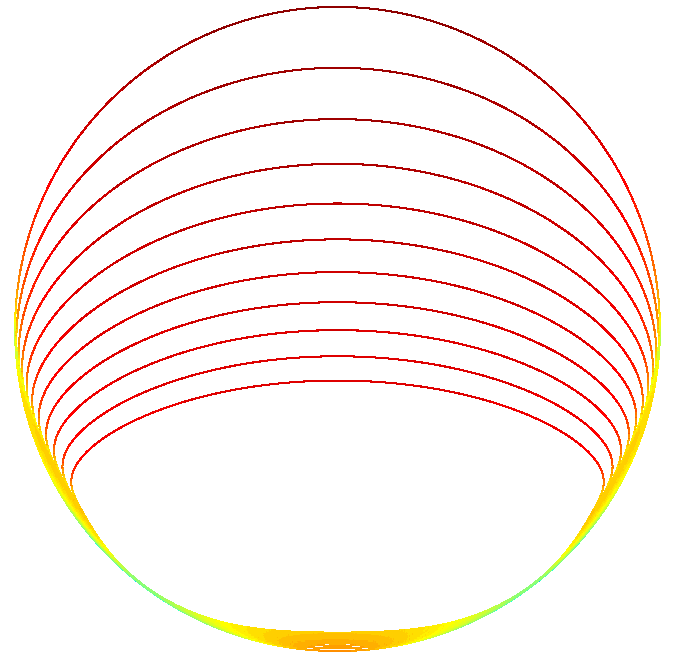
\includegraphics[width = 0.30 \textwidth]{./figs/1b_0d4r1h_shear}
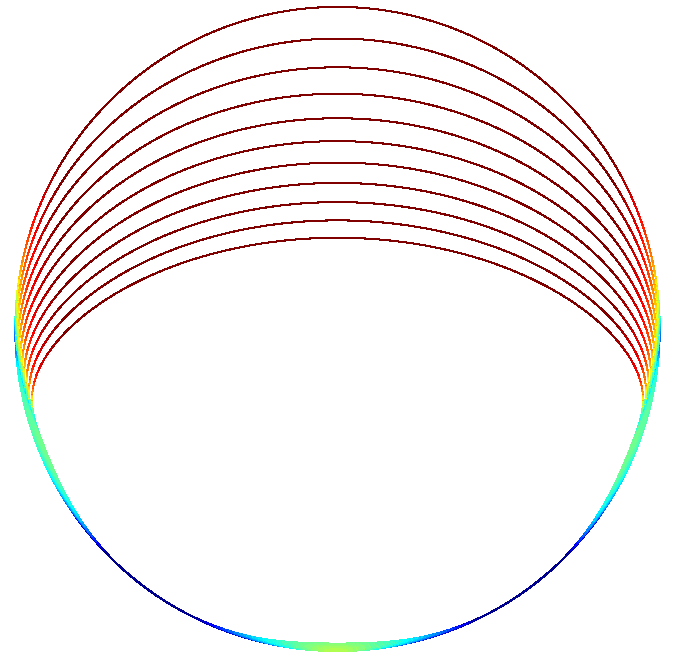
\includegraphics[width = 0.30 \textwidth]{./figs/1b_0d4r0d5h_shear}
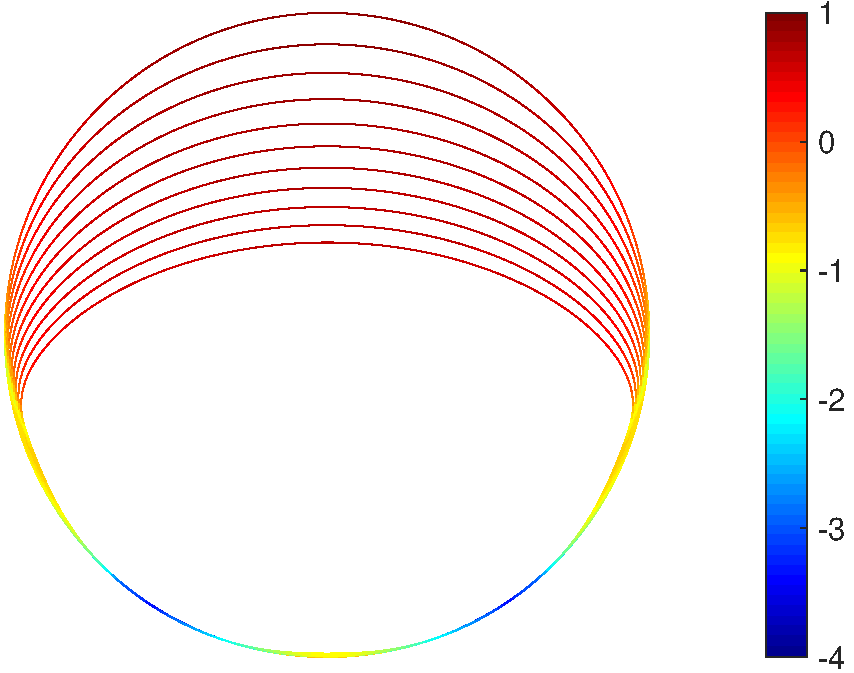
\includegraphics[width = 0.35 \textwidth]{./figs/1b_0d4r0d1h_shear}
\caption{A single body eroding in Stokes flow. Color indicates the shear stress on the body. In this simulation, we use three minimum body-to-wall initial distances $d=h$(left), $h/2$(middle), and $h/10$(right) with $N_\iin = 256$ discretization points on the body, $N_\out = 1024$ points on the outer boundary, a time-step of $\Dt$, and smoothing parameters of $\eps $ and $\sigma $.}
\label{} 
\end{center}
\end{figure}
{\color{red} We first consider a single circular body in a shear flow. The domain $\Omega$ is a rectangle $[-3,3]\times[-1,1]$ with rounded corners. The velocity of flow from the left side of $\Omega$ is $v(x_1,x_2)=x_2+1$. Let the radius of the body be $r$, the length of the body be $L$, $N_\iin$ and $N_\out$ be the number of discretization points on the body and wall respectively, $h=L/N_\iin$ be the resolution mesh size of the body, and $d$ be the minimum initial distance from body to wall. 
To investigate the shape of eroding body when it is close to wall, we set $r=0.4$, $N_\iin=256$, and $N_\out=1024$ with respect to three different $d=h, h/2$, and $ h/10$. 

}
%%%%%%%%%%%%%%%%%%%%%%%%%%%%%%%%%%%%%%%%%%%%%%%%%%%%%%%%%%%%%%%%%%%%%%%

\begin{figure}[H]
\begin{center}
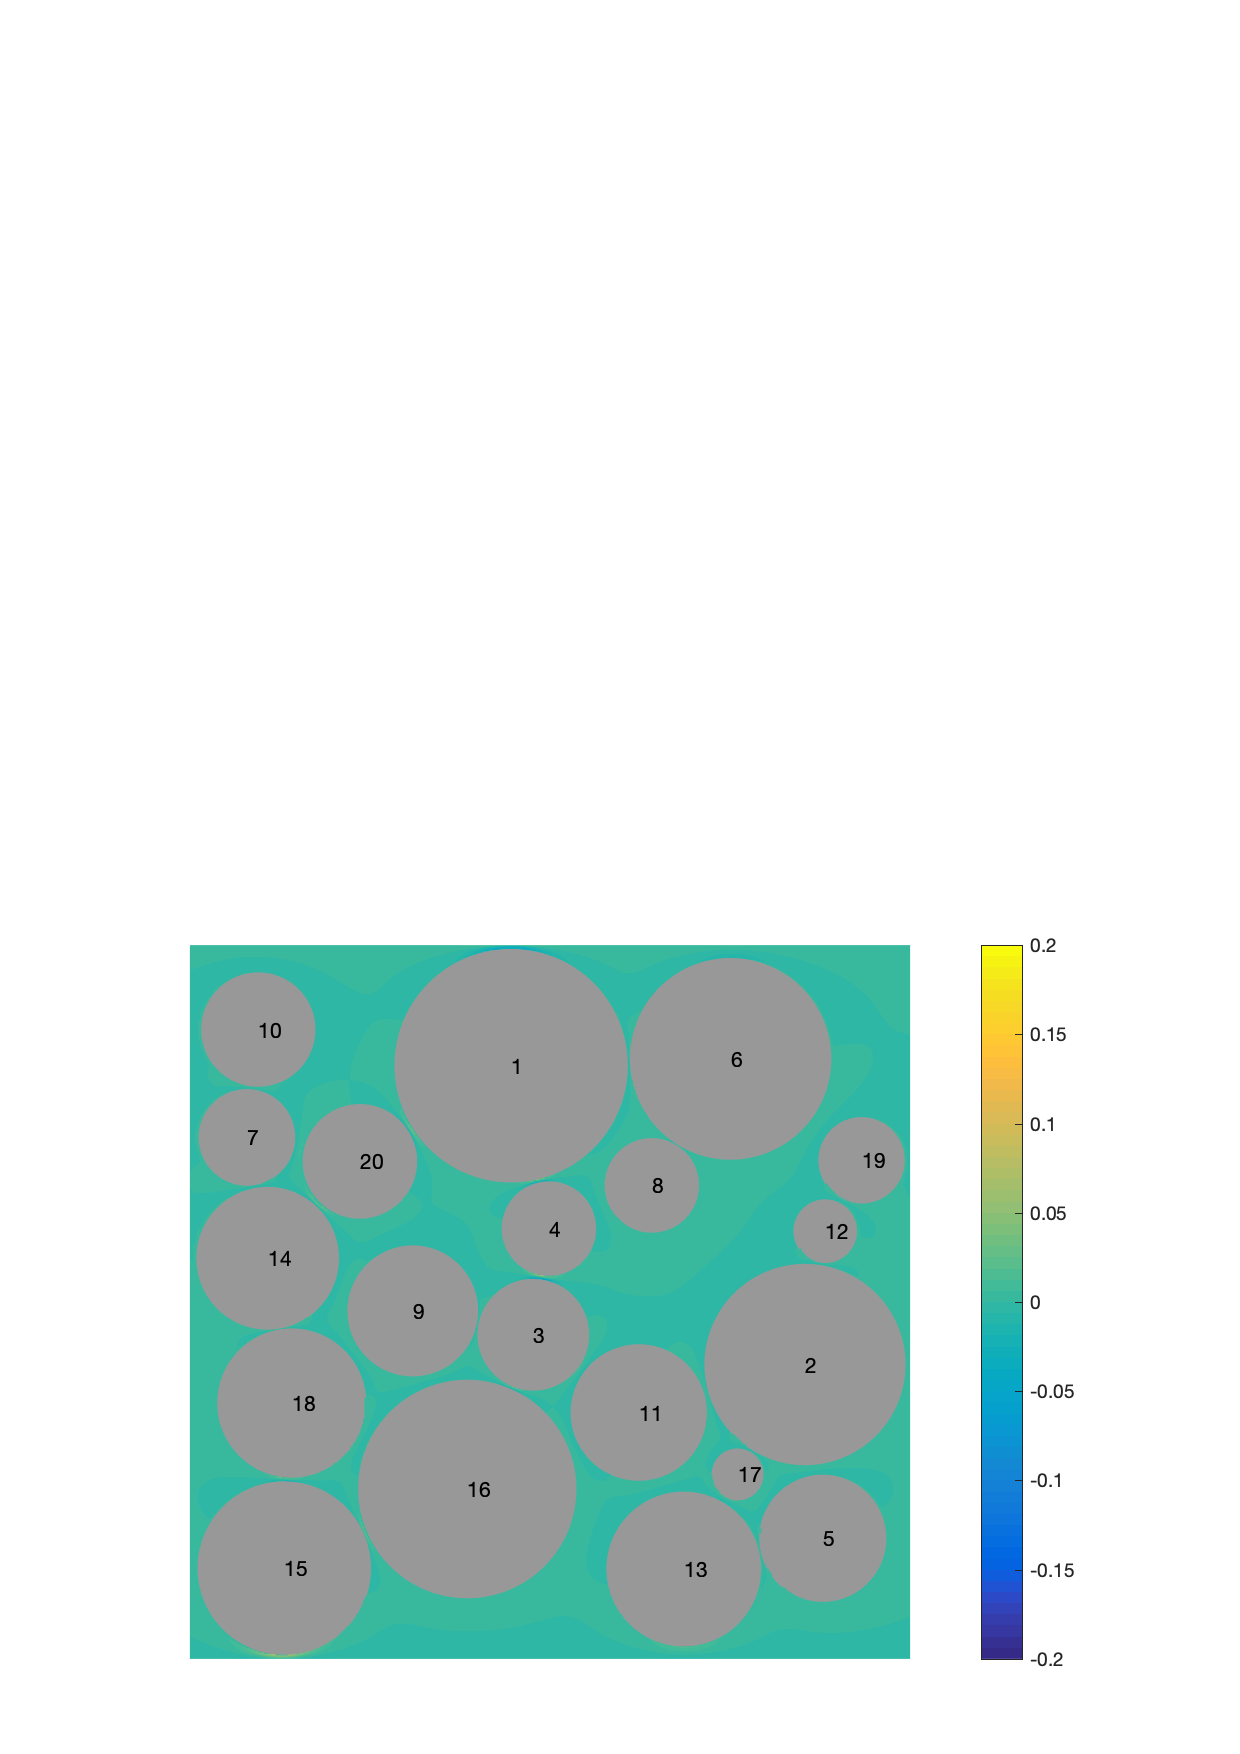
\includegraphics[width = 0.42 \textwidth]{./figs/20b_dense_1}
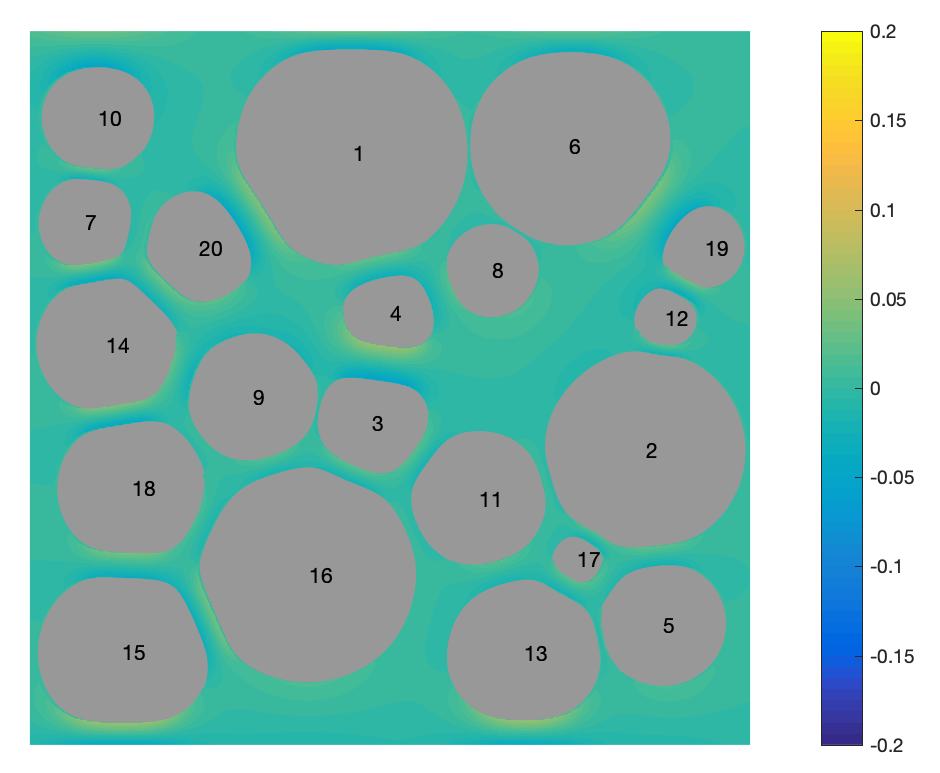
\includegraphics[width = 0.507 \textwidth]{./figs/20b_dense_101}\\

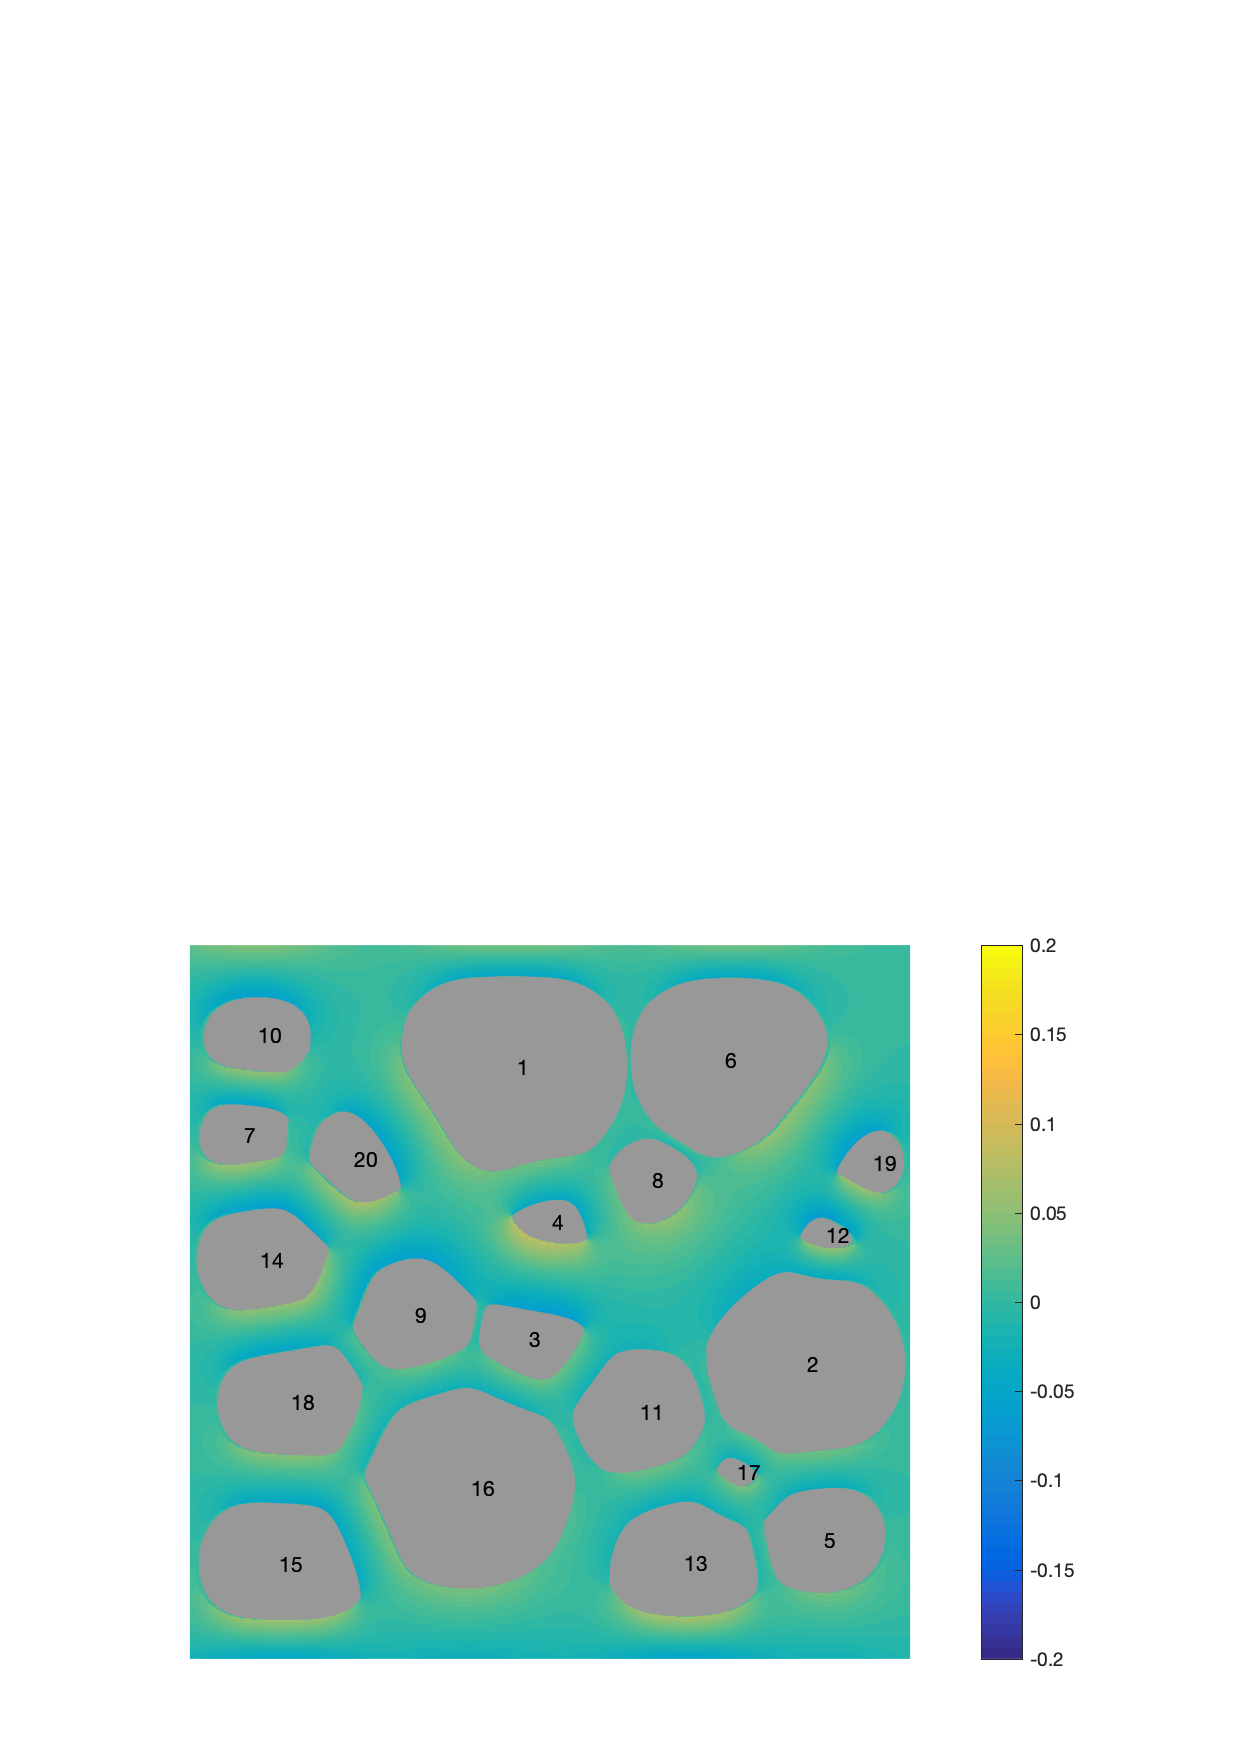
\includegraphics[width = 0.42 \textwidth]{./figs/20b_dense_201}
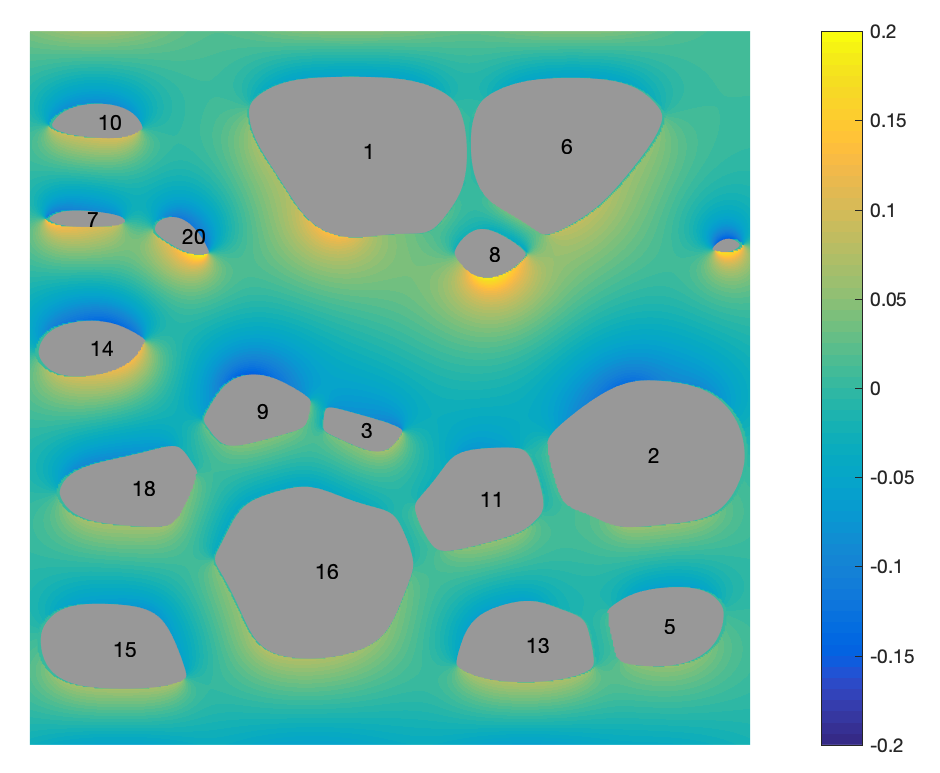
\includegraphics[width = 0.507 \textwidth]{./figs/20b_dense_301}
\caption{Erosion of 20 nearly touching bodies with the fixed-pressure-drop condition. The color is the vorticity of fluid. The 4 snapshots are evenly spaced in time. In this simulation, we use $N_\iin = 256$ discretization points on the body, $N_\out = 1024$ points on the outer boundary, a time-step of $\Dt=10^{-4}$, and smoothing parameters of $\eps $ and $\sigma $.}
\label{} 
\end{center}
\end{figure}
\subsection{20 nearly touching bodies}
{\color{red} 
By using Barycentric quadrature rule, we are able to capture the details in the fluid when wall and bodies or body and bodies are close to each other. The first nearly touching bodies case is 20 bodies in a Hagen-Poiseuille flow. The domain $\Omega$ is a rectangle $[-3,3]\times[-1,1]$ with rounded corners. The velocity of flow from the left side of $\Omega$ is $v(x_1,x_2)=(1+x_2)(1-x_2)$. The number of discretization points $N_\iin$ on the bodies is 256 and the number of discretization points $N_\out$ on the outer boundary is 1024. 
}

\begin{figure}[H]
\begin{center}
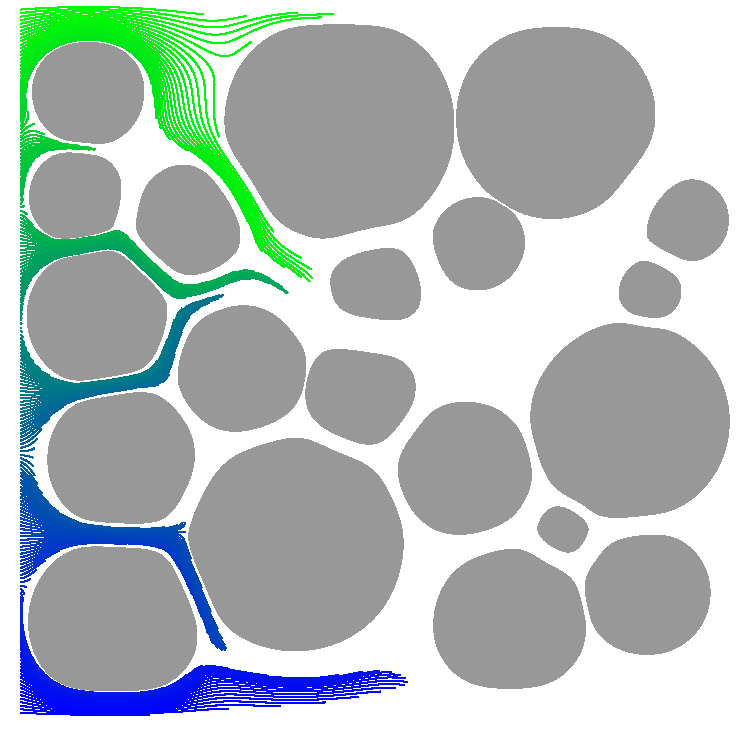
\includegraphics[width = 0.3 \textwidth]{./figs/tracer_20b30}
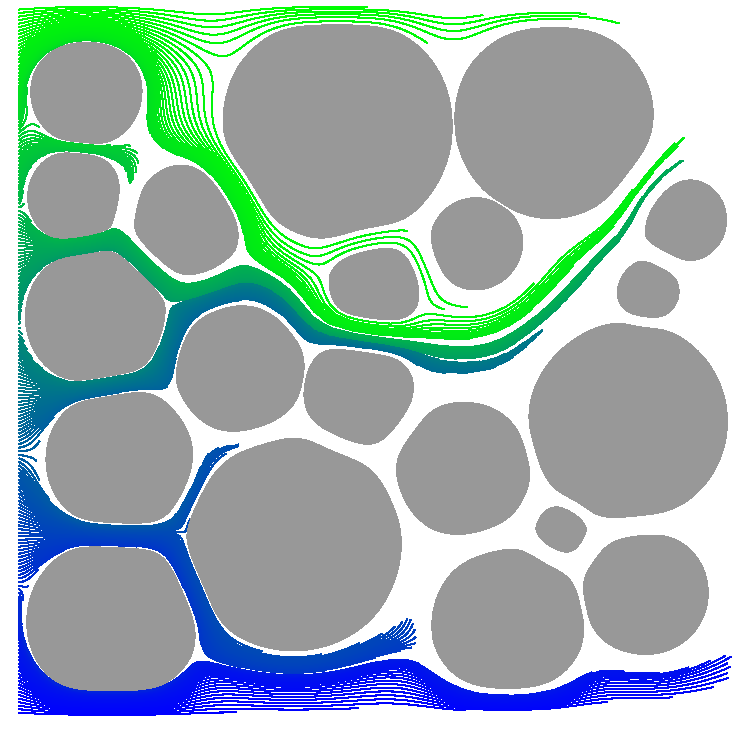
\includegraphics[width = 0.3 \textwidth]{./figs/tracer_20b60}
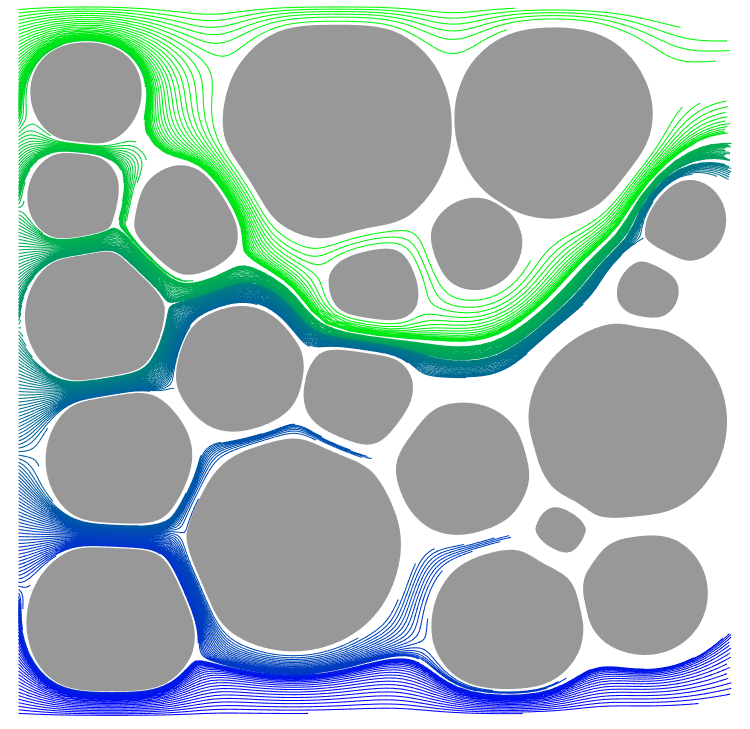
\includegraphics[width = 0.3 \textwidth]{./figs/tracer_20b90}\\

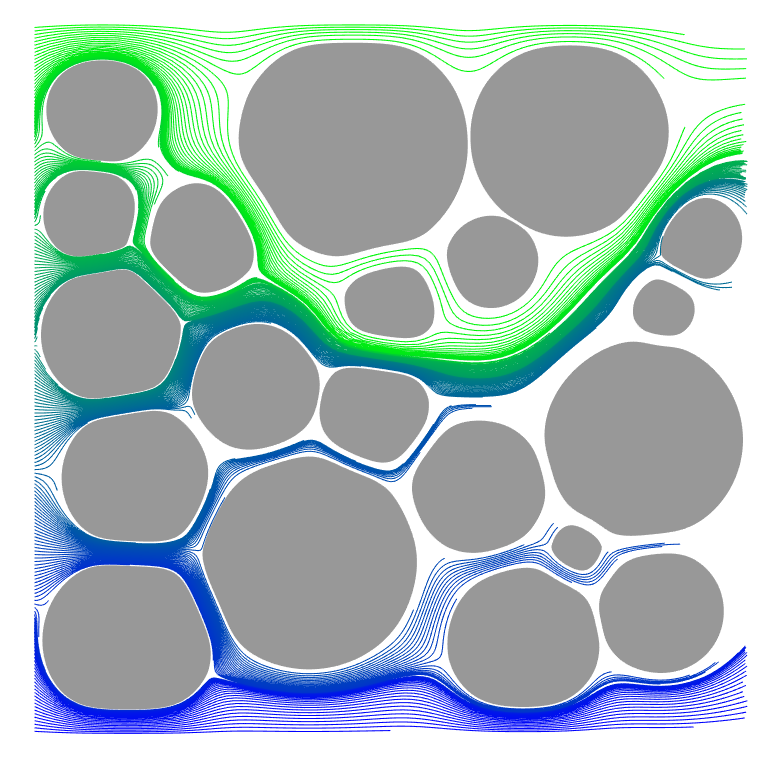
\includegraphics[width = 0.3 \textwidth]{./figs/tracer_20b120}
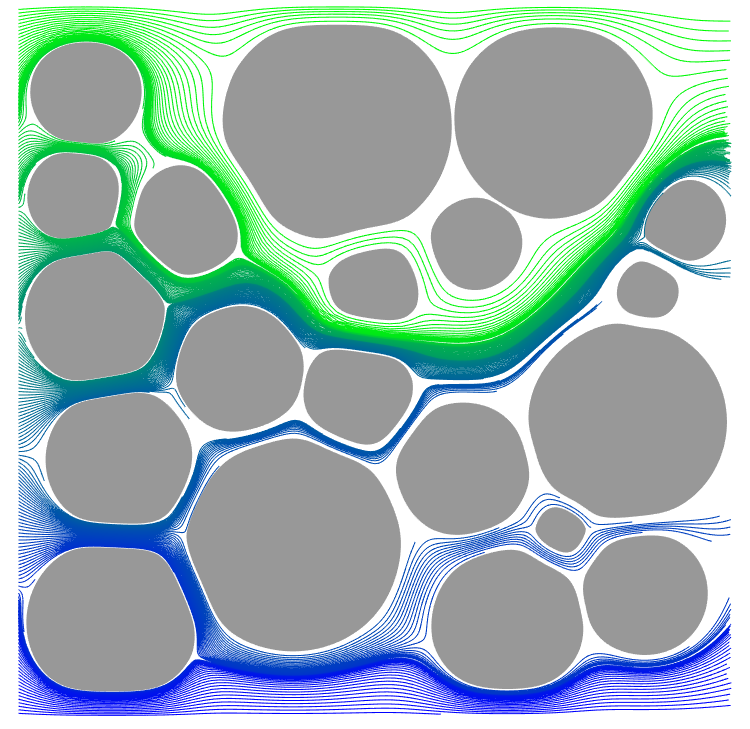
\includegraphics[width = 0.3 \textwidth]{./figs/tracer_20b150}
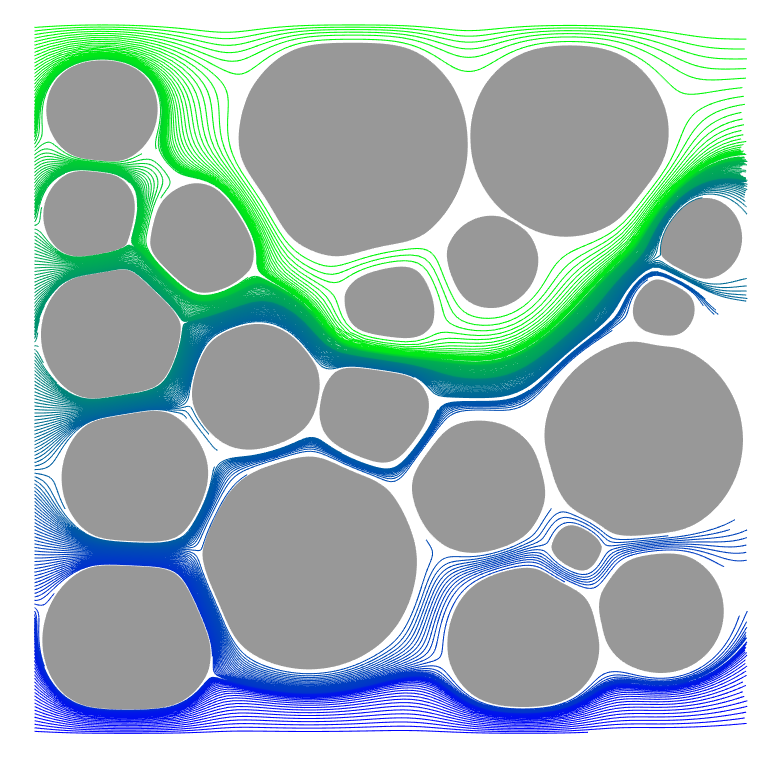
\includegraphics[width = 0.3 \textwidth]{./figs/tracer_20b180}\\

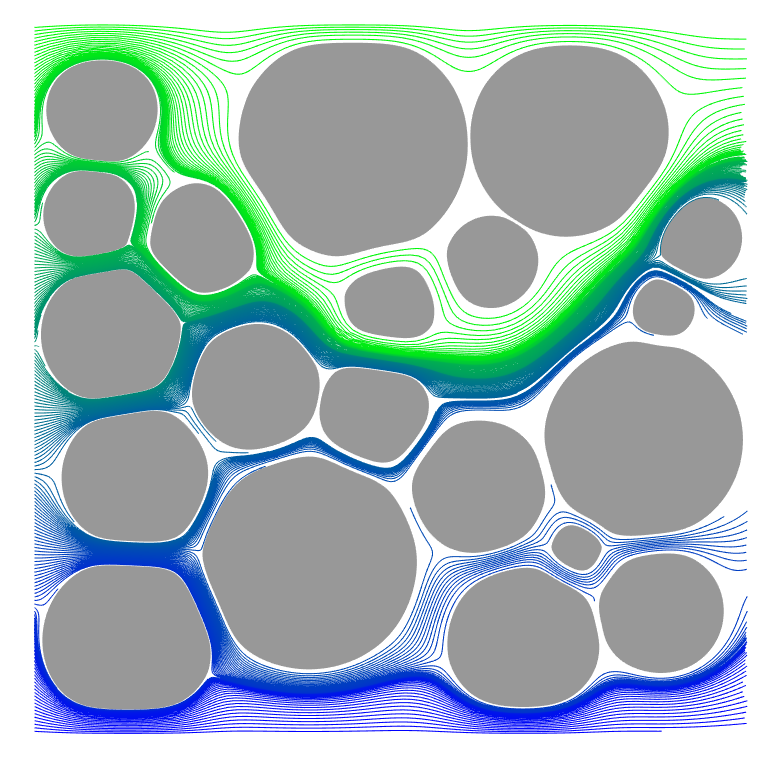
\includegraphics[width = 0.3 \textwidth]{./figs/tracer_20b210}
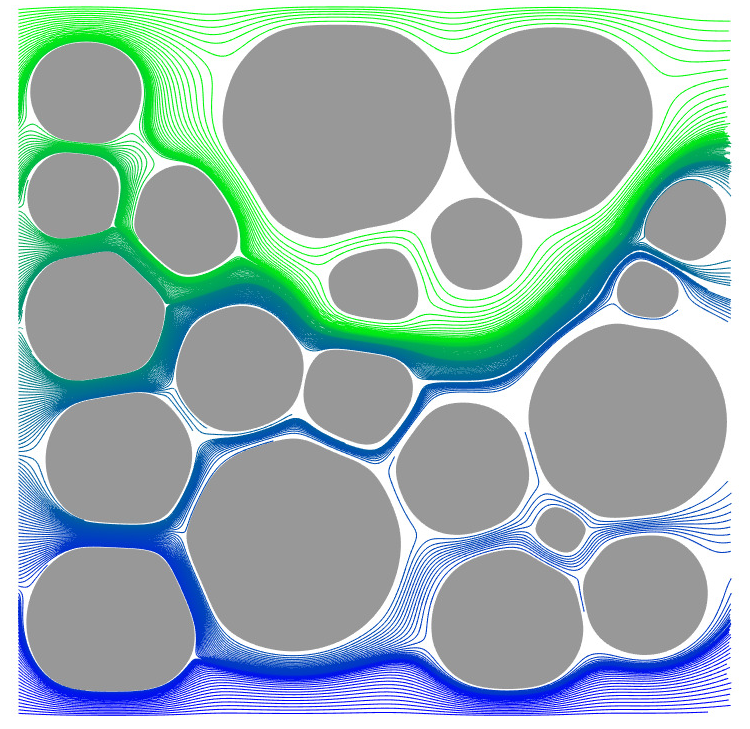
\includegraphics[width = 0.3 \textwidth]{./figs/tracer_20b240}
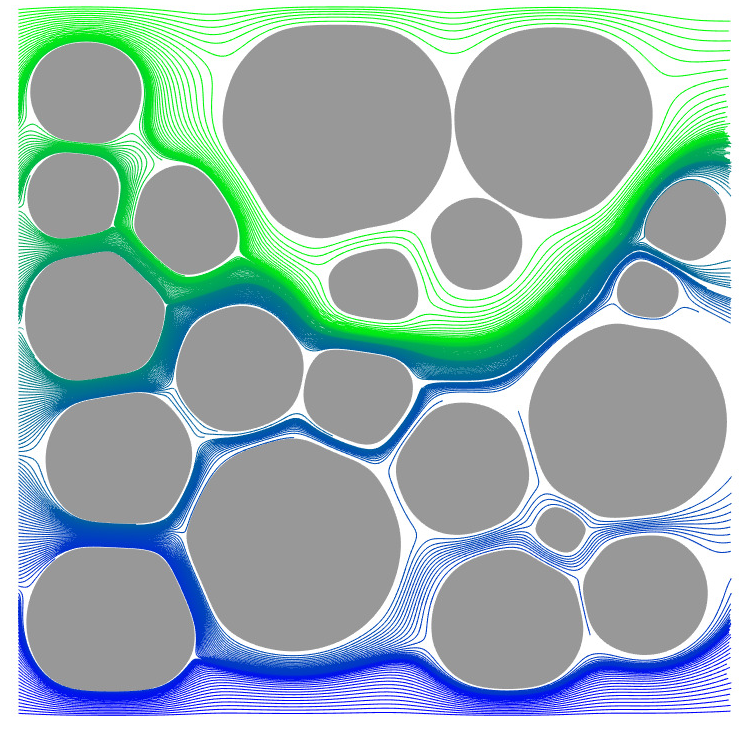
\includegraphics[width = 0.3 \textwidth]{./figs/tracer_20b270}
\caption{The trajectories of tracers in the fluid with 20 bodies. The 9 snapshots are evenly spaced in time.}
\end{center}
\end{figure}

\begin{figure}[H]
\begin{center}
\caption{The tortuosity of the 20 nearly touching bodies}
\end{center}
\end{figure}

%%%%%%%%%%%%%%%%%%%%%%%%%%%%%%%%%%%%%%%%%%%%%%%%%%%%%%%%%%%%%%%%%%%%%%%
\subsection{50 nearly touching bodies}
{\color{red}
The second nearly touching bodies case is 50 bodies in a Hagen-Poiseuille flow.
}
%%%%%%%%%%%%%%%%%%%%%%%%%%%%%%%%%%%%%%%%%%%%%%%%%%%%%%%%%%%%%%%%%%%%%%%
\section{Conclusions}
\label{s:conclusions}
%%%%%%%%%%%%%%%%%%%%%%%%%%%%%%%%%%%%%%%%%%%%%%%%%%%%%%%%%%%%%%%%%%%%%%%


%%%%%%%%%%%%%%%%%%%%%%%%%%%%%%%%%%%%%%%%%%%%%%%%%%%%%%%%%%%%%%%%%%%%%%%
\paragraph{\bf Acknowledgments} We would like to thank Manas Rachh for
supplying the FMM for the Stokes double-layer potential. BQ and NM were
supported by Florida State University startup funds and Simons
Foundation Mathematics and Physical Sciences-Collaboration Grants for
Mathematicians.

\bibliographystyle{plainnat} 
\biboptions{sort&compress}
\bibliography{refs}


\end{document}








%old stuff%
%%%%%%%%%%%%%%%%%%%%%%%%%%%%%%%%%%%%%%%%%%%%%%%%%%%%%%%%%%%%%%%%%%%%%%%%
%\subsection{boundary integral equation formulation} 
%\label{sec:bies}
%add an introduction why we do not use the double-layer potentials of stokes equations but the double-layer potentials of laplace equations to solve stokes equation when we use barycentric approach (or complex variable approach).
%
%\subsubsection{laplace's equations from $\rdb^2$ to $\cdb$ }
%
%let $\omega$ be the domain of fluid. the boundary of $\omega$ is $\gamma$ and the outward normal vector on $\gamma$ is ${\bf n_y}=(n_1,n_2)$.
%
%consider a laplace's equations with dirichlet boundary condition
%\begin{equation}\label{laplace}
%  \begin{cases}
%    \delta {\bf u}=0, & \text{in}\,\,\, \omega \in \rdb^2;\\
%    {\bf u}={\bf f}, & \text{on}\,\,\, \gamma.
%  \end{cases}
%\end{equation}
%
%Let ${\bf x}=(x_1,x_2), {\bf y}=(y_1,y_2)$. Then we have ${\bf r}={\bf x} - {\bf y}$ and $\rho=|\bf r|$.
%The double-layer potential which solves \eqref{Laplace} is 
%\begin{align*}
%\D[\sigma]({\bf x})&=\frac{1}{2\pi}\displaystyle\int_{\Gamma} \frac{{\bf r} \cdot {\bf n_y}}{\rho^2}\sigma({\bf y})ds_y,
%%\frac{1}{2\pi}\displaystyle\int_{\Gamma}\frac{\partial}{\partial {\bf n_y}} \log |{\bf x}-{\bf y}| \sigma({\bf y})ds_y,\\ \\
%%&=\frac{-1}{2\pi}\int_{\Gamma}\frac{{\bf r}\cdot{\bf n_y}}{\rho^2} \sigma({\bf y})ds_y\\ \\
%%&=\frac{-1}{2\pi}\int_{\Gamma}\frac{n_1(x_1-y_1)+n_2(x_2-y_2)}{(x_1-y_1)^2+(x_2-y_2)^2} \sigma({\bf y})ds_y 
%\numberthis\label{DLP:real}
%\end{align*}
%where $\sigma$ is the density function on the boundary $\Gamma$.
%
%
%Consider a Cauchy integral 
%\begin{equation}\label{CI}
%v({x})=\frac{1}{2\pi i}\int_{\Gamma}\frac{\sigma({ y})}{{ y}-{ x}} d{ y},\,\,\,\,\,\,\,\,\, \forall { x} \in \Cdb\setminus \Gamma.
%\end{equation}
%where ${ x}=x_1+ix_2$, $ { y}=y_1+iy_2$, ${ n_y}=n_1+i n_2$ and $d{ y}=i {n_y}ds_y$. It can be shown that 
%the real part of the Cauchy integral in \eqref{CI} is equivalent to the double-layer potential in \eqref{DLP:real}. 
%
%
%\subsubsection{From Stokes DLP to Laplace DLPs}
%
%Let ${\bf x}=(x_1,x_2), {\bf y}=(y_1,y_2)$. Then we have ${\bf r}={\bf x} - {\bf y}$ and $\rho=|\bf r|$.
%
%
%The Stokes double-layer potential  is
%\begin{equation}\label{StokesDLP1}
%\D[\boldsymbol\sigma]({\bf x}):=\frac{1}{\pi}\int_{\Gamma}\left(\frac{{\bf r} \cdot {\bf n_y}}{\rho^2}\frac{{\bf r} \otimes {\bf r}}{\rho^2}\right) {\boldsymbol\sigma({\bf y})} d s_y.
%\end{equation}
%We could rewrite the Stokes DLP in terms of the Laplace DLP as
%\begin{align*}\label{StokesDLP2}
%\D[\boldsymbol\sigma]({\bf x})=\frac{1}{2\pi}\int_{\Gamma}&\frac{{\bf n_y}}{\rho^2}({\bf r} \cdot {\boldsymbol \sigma})ds_y+\frac{1}{2\pi}\nabla\int_{\Gamma}\frac{{\bf r} \cdot {\bf n_y}}{\rho^2}({\bf y} \cdot{\boldsymbol \sigma})ds_y\\
%&-\frac{1}{2\pi}x_1 \nabla\int_{\Gamma}\frac{{\bf r} \cdot {\bf n_y}}{\rho^2}\sigma_1ds_y-\frac{1}{2\pi}x_2\nabla\int_{\Gamma}\frac{{\bf r} \cdot {\bf n_y}}{\rho^2}\sigma_2ds_y. \numberthis
%\end{align*}
%

 
%%%%%%%%%%%%%%%%%%%%%%%%%%%%%%%%%%%%%%%%%%%%%%%%%%%%%%%%%%%%%%%%%%%%%%%%
%\subsection{Computing the shear stress}
%\label{sec:shearStressLP}
%
%To calculate the shear stress, we need to know the gradient of double-layer potential in \eqref{StokesDLP2} 
%\begin{align*}\label{SSLP}
%\nabla\D[\boldsymbol\sigma]({\bf x})=\frac{1}{2\pi}\nabla\int_{\Gamma}&\frac{{\bf n_y}}{\rho^2}({\bf r} \cdot {\boldsymbol \sigma})ds_y+\frac{1}{2\pi}\nabla^2\int_{\Gamma}\frac{{\bf r} \cdot {\bf n_y}}{\rho^2}({\bf y} \cdot{\boldsymbol \sigma})ds_y\\
%&-\frac{1}{2\pi}\nabla\left(x_1 \nabla\int_{\Gamma}\frac{{\bf r} \cdot {\bf n_y}}{\rho^2}\sigma_1ds_y\right)-\frac{1}{2\pi}\nabla\left(x_2\nabla\int_{\Gamma}\frac{{\bf r} \cdot {\bf n_y}}{\rho^2}\sigma_2ds_y\right). \numberthis
%\end{align*}
%
%
%
%
%%%%%%%%%%%%%%%%%%%%%%%%%%%%%%%%%%%%%%%%%%%%%%%%%%%%%%%%%%%%%%%%%%%%%%%%
%\subsection{Boundary evolution in the {\thL} framework} 
%\label{sec:thetaL}
%
%
%%%%%%%%%%%%%%%%%%%%%%%%%%%%%%%%%%%%%%%%%%%%%%%%%%%%%%%%%%%%%%%%%%%%%%%%
%\subsection{Solving the BIE}
%\label{sec:BIE}
%\subsubsection{Interior Case}
%Consider a Cauchy integral 
%\begin{align}\label{CIFI}
%\frac{1}{2\pi i}\int_{\Gamma}\frac{v^-({ y})}{{ y}-{ x}} d{ y}
%&=\begin{cases}
%\,v(x), &{ x} \in \Omega,\\ 
%\,0,  &{ x} \in \Cdb\setminus \bar{\Omega}.
%\end{cases}
%\end{align}
%By the identity of Cauchy Integral Formula $\displaystyle\frac{1}{2 \pi i}\int_{\Gamma}\frac{1}{{ y}-{ x}} d{ y}=1,$ we can rewrtie \eqref{CIFI} and get 
%\begin{equation}
%\frac{1}{2\pi i}\int_{\Gamma}\frac{v^-({ y})-v(x)}{{ y}-{ x}} d{ y}=0,\,\,\,\,\,\,\,\,\, \forall { x} \in \Omega.
%\end{equation}
%\begin{equation}\label{dNCI}
%v'({x})=\frac{1}{2\pi i}\int_{\Gamma}\frac{v^-({ y})}{(y- x)^2} d{ y},\,\,\,\,\,\,\,\,\, \forall { x} \in \Omega.
%\end{equation}
%By the identity of Cauchy Integral Formula $\displaystyle\frac{1}{2 \pi i}\int_{\Gamma}\frac{1}{( y- x)^n} d{ y}=0$ for integer n $\neq 1$, we can rewrtie \eqref{dNCI} and get 
%\begin{equation}
%\frac{1}{2\pi i}\int_{\Gamma}\frac{v^-({ y})-v(x)-(y-x)v'(x)}{(y-x)^2} d{ y}=0,\,\,\,\,\,\,\,\,\, \forall { x} \in \Omega.
%\end{equation}
%
%\subsubsection{Exterior case}
%Consider a Cauchy integral formula for the exterior domain
%\begin{align}\label{CIFE}
%\frac{1}{2\pi i}\int_{\Gamma}\frac{v^+({ y})}{{ y}-{ x}} d{ y}
%&=\begin{cases}
%\,v_{\infty}, &{ x} \in \Omega,\\ 
%\,-v(x)+v_{\infty},  &{ x} \in \Omega^c,
%\end{cases}
%\end{align}
%where $v_{\infty}=\displaystyle\lim_{x \to \infty}v(x)$.
%\begin{equation}
%\frac{1}{x-a}=\frac{-1}{2 \pi i} \int_{\Gamma}\frac{(y-a)^{-1}}{y-x} d{ y},\,\,\,\,\,\,\,\,\, \forall { x} \in \Omega^c.
%\end{equation}
%\begin{equation}
%\frac{1}{2\pi i}\int_{\Gamma}\frac{v^+({ y})-(y-a)^{-1}(x-a)v(x)}{y-x} d{ y}=0,\,\,\,\,\,\,\,\,\, \forall { x} \in \Omega^c.
%\end{equation}
%\begin{equation}
%\frac{1}{2\pi i}\int_{\Gamma}\frac{v^+({ y})-v(x)-(y-a)^{-1}(x-a)(y-x)v'(x)}{(y-x)^2} d{ y}=0,\,\,\,\,\,\,\,\,\, \forall { x} \in \Omega^c.
%\end{equation}
%
%%%%%%%%%%%%%%%%%%%%%%%%%%%%%%%%%%%%%%%%%%%%%%%%%%%%%%%%%%%%%%%%%%%%%%%%
%\subsection{Shear stress}
%\label{sec:shearStress}
%\subsubsection{Interior Case}
%\begin{equation}\label{ddNCI}
%v''({x})=\frac{1}{2\pi i}\int_{\Gamma}\frac{2v^-({ y})}{(y- x)^3} d{ y},\,\,\,\,\,\,\,\,\, \forall { x} \in \Omega.
%\end{equation}
%By the identity of Cauchy Integral Formula $\displaystyle\frac{1}{2 \pi i}\int_{\Gamma}\frac{1}{( y- x)^n} d{ y}=0$ for integer n $\neq 1$, we can rewrtie \eqref{ddNCI} and get 
%\begin{equation}
%\frac{1}{2\pi i}\int_{\Gamma}\frac{2v^-({ y})-2v(x)-2(y-x)v'(x)-(y-x)^2v''(x)}{(y-x)^3} d{ y}=0,\,\,\,\,\,\,\,\,\, \forall { x} \in \Omega.
%\end{equation}
%\subsubsection{Exterior case}
%\begin{equation}
%\frac{1}{2\pi i}\int_{\Gamma}\frac{2v^+({ y})-2v(x)-2(y-x)v'(x)-(y-a)^{-1}(x-a)(y-x)^2v''(x)}{(y-x)^3} d{ y}=0,\,\,\,\,\,\,\,\,\, \forall { x} \in \Omega^c.
%\end{equation}
%%%%%%%%%%%%%%%%%%%%%%%%%%%%%%%%%%%%%%%%%%%%%%%%%%%%%%%%%%%%%%%%%%%%%%%%
%%% TIME-STEPPING %%
%\subsection{Time-stepping with the {\thL} method} 
%\label{sec:timeStepping}
%
%
%%%%%%%%%%%%%%%%%%%%%%%%%%%%%%%%%%%%%%%%%%%%%%%%%%%%%%%%%%%%%%%%%%%%%%%%
%\section{Post processing quantities of interest}
%\label{s:qoi}
%
%%%%%%%%%%%%%%%%%%%%%%%%%%%%%%%%%%%%%%%%%%%%%%%%%%%%%%%%%%%%%%%%%%%%%%%%
%\subsection{Vorticity}
%%%%%%%%%%%%%%%%%%%%%%%%%%%%%%%%%%%%%%%%%%%%%%%%%%%%%%%%%%%%%%%%%%%%%%%%
%\subsection{Pressure}
%\label{sec:pressure}
%
%%%%%%%%%%%%%%%%%%%%%%%%%%%%%%%%%%%%%%%%%%%%%%%%%%%%%%%%%%%%%%%%%%%%%%%%
%\subsection{Drag}
%\label{sec:drag}
%
%%%%%%%%%%%%%%%%%%%%%%%%%%%%%%%%%%%%%%%%%%%%%%%%%%%%%%%%%%%%%%%%%%%%%%%%
%\subsection{Near-singular integration}
%\label{sec:NSI}
%

